\subsection{REST and RESTful services}

\subsubsection{What is the REST?}
Representational state transfer (REST) is a software design model for
distributed systems~\cite{Fielding2000}. This term was introduced in 2000 in the doctoral dissertation of
Roy Fielding, one of the principal authors of the Hypertext Transfer Protocol
(\gls{HTTP}) specification. REST uses a stateless, client-server,
cacheable communications protocol which is almost always the HTTP protocol. Its original
feature is to work by using simple HTTP to make calls between machines instead
of choosing more complex mechanisms such as CORBA, RPC or SOAP.

REST-style architectures conventionally consist of clients and servers.
Clients make requests to servers, servers process requests and return responses.
Requests and responses are built around the transfer of \textit{representations}
of \textit{resources}.
Author defines the resource as the key abstraction of information in
REST~\cite{Fielding2000}. It can be any information that can be named and
addressed: documents, images, non-virtual physical systems and services.
A representation of a resource is typically a document that captures the current or intended state of a resource.

Restful applications use HTTP requests to change a state of resource  \footnote{
all four CRUD(Create/Read/Update/Delete) operations)}: post data to create and/or update
resource, read data (e.g., make queries) to get current state of resource, and
delete data to delete existing resource.

REST does not offer security features, encryption, session management, QoS
guarantees, etc. But these can be added by building on top of HTTP, for example
username/password tokens are often used for encryption, REST can be used on
top of HTTPS (secure sockets)\cite{ws_techologies_state_of_the_art}.

\subsubsection{Key principles of REST}
REST is a set of principles that define how Web standards, such as HTTP and
\gls{URI}s, are supposed to be used.

The  five key principles of REST are\cite{rest_brief_intro}:
\begin{itemize}
  
 \item Give every “thing” an ID
 \item Link things together
 \item Use standard methods
 \item Resources with multiple representations
 \item Communicate statelessly
  
\end{itemize}

\paragraph{Give every “thing” an ID}  ~\\

Every resource need to be reachable and identifiable. You need to access it
somehow, therefore you need an identificator for the resource. World Wide Web
uses \gls{URI} identificators for that purpuse. Resource \gls{URI} could look like:

\begin{listing}[H]
\begin{minted}[frame=lines,
               framesep=2mm]{html}
http://example.com/customers/1234
http://example.com/orders/2007/10/776654
http://example.com/products/4554
http://example.com/processes/salary-increase-234 
http://example.com/orders/2007/11
http://example.com/products?color=green
\end{minted}
\caption{Resource identificator examples \cite{rest_brief_intro}}
\label{lst:uri_example}
\end{listing}

URIs identify resources in a global namespace. This means that this
identificator should be unique and there should not be another same URI.
This URI may reflect a defined customer, order or product and it might correspond
to database entry. \autoref{lst:uri_example} last two examples identify more
than one thing. They identify a collection of objects, which is the object
itself and require an identificator.

\paragraph{Link things together}  ~\\

Previous principle introduced an unigue global identificator for the resource.
Resource URI gives posibility to access the resource from different locations
and applications. Resources can be also linked to each other.
Listing \ref{lst:linked_uri_example} shows such scheme. Representation of an
order contains the information about this order and linked product and client resources.
This approach gives client an opportunity to change a state of client application by following linked
resources. After receiving order information client has two possibilities for
choice: to get product information or to fetch customer details. 

\begin{listing}[H]
\begin{minted}[frame=lines,
               framesep=2mm]{xml}
<order self='http://example.com/orders/2007/10/776654' > 
   <amount>23</amount> 
   <product ref='http://example.com/products/4554' /> 
   <customer ref='http://example.com/customers/1234' /> 
</order> 
\end{minted}
\caption{Example of linked resources\cite{rest_brief_intro}}
\label{lst:linked_uri_example}
\end{listing}
 
The idea of links is a core principle of the Web~\footnote{The World Wide Web
(abbreviated as WWW or W3,[3] commonly known as the web), is a system of
interlinked hypertext documents accessed via the Internet.\cite{wikipedia:WWW}}

\paragraph{Use standard methods} ~\\

There should be a standard inteface for accessing the resource object.
REST relies on HTTP protocol, which has definitions of some standard request
methods:
GET, PUT, POST and DELETE.
\autoref{tbl:rest_http_api} describes standard actions on resource.

\begin{table}[h]
	\centering	
	\begin{tabularx}{\textwidth}{|X|X|X|X|X|}
		\hline
		\textbf{Resource} & 
		\textbf{GET}  	& 
		\textbf{PUT} 	&
		\textbf{POST} &
		\textbf{DELETE}
	    
	    \tabularnewline
		\hline
			\begin{sloppypar}
				\textbf{Collection URI, such as \url{http://example.com/resources}}
			\end{sloppypar} &
			\textbf{List} the URIs and perhaps other details of the collection's members.&
			\textbf{Replace} the entire collection with another collection.&
			\textbf{Create} a new entry in the collection. The new entry's URI is
			assigned automatically and is usually returned by the operation. &
			\textbf{Delete} the entire collection.
			
	    	\tabularnewline	    	
	    	\hline
	    	\begin{sloppypar}
				\textbf{Element URI, such as \url{http://example.com/resources/item17}} 
			\end{sloppypar} &
			\textbf{Retrieve} a representation of the addressed member of the
			collection, expressed in an appropriate Internet media type. &
			\textbf{Replace} the addressed member of the collection, or if it
			doesn't exist, \textbf{create} it. &			
			Not generally used. Treat the addressed member as a collection in its own
			right and \textbf{create} a new entry in it. &			
			\textbf{Delete} the addressed member of the collection.
	
	    \tabularnewline
		\hline	  
	\end{tabularx} 
	\caption{RESTful web API HTTP methods \cite{wikipedia:REST}}
	\label{tbl:rest_http_api}
\end{table}

All four \gls{CRUD} operations may be done with these HTTP methods. It is
possible to manage a whole lifecycle using only these methods. Client of the
service should only implement   the default application protocol (HTTP)
in correct way.

\paragraph{Resources with multiple representations} ~\\
\label{sec:rest_multiple_resource_types}
When client gets representation of a resource using GET method he does not know
which data format will server return. REST as architectural method does not
provide any special standard for resource representation. How can client and
server could make an agreement about data format they will use?


HTTP protocol help to solve these problems again. 
It has a special field that defines the operating parameters of an HTTP
transaction. Field \textif{Accept} in the header of HTTP request message
specifies content type that is acceptable for the response~\cite{http-rfc}.

Such request header could look like this:

\begin{listing}[H]
\begin{minted}[frame=lines,
               framesep=2mm]{html}
GET /images/567 HTTP/1.1
Host: example.com
Accept: image/jpeg
\end{minted}
\caption{Request for a representation of resource in a particular format}
\label{lst:http_accept_example}
\end{listing}

This means that client expects that representation of a resource having
identificator \url{http://www.example.com/images/567} should be in
\textit{image/jpeg} format. Both client and server should be aware of such
format, whole system may be designed around any special format. 
There could be also an another representation of same resouce( the same image),
for example \textit{image/png} or \textit{image/bmp} formats, that server could
send according to received request. 

Not only outgoing data format could be specified. Server can also consume data
in specific formats (there are different specific header fields for this, for
example \textit{Content-Type}).

Using multiple representations of resources helps to connect more possible
clients to the system.

\paragraph{Communicate statelessly} ~\\

Stateless communication helps to design more scalable systems.
RESTful server does not  keep any communication context. Each incoming  request
is new for the server and there should be enough information to necessary to
understand the request\cite{Fielding2000}.

Server could contain all the information about each connected client, but it
requires a meaningful amount of resources. Server need to keep and control the
current state of application for every client, which locks the server resources
while client is not active (opened connections, memory, data integrity locks).

There is no need for keeping using all these resources if the application state
is on the client side. Client controls the flow of the application and
changes its state by making requests to server. Server does not make any work
while clients are not sending requests, it starts to work only on demand.

You can easilly switch between different servers if there is no any client
context on the server side. Imagine a system with some amount of application
servers and load balancer server in it. All application servers run the same
application. While some servers are making hard work, another servers may be
idle.
Load balancer have a posibility to route new incoming requests to a server,
which has a smallest workload, because of the absence of application context
between client and server. Even parallel request of the same client could be
handled by different servers. Such system become more scalable and new server
nodes can be easilly added or removed.

The main disadvantage of such approach is the decrease of network performance.
Client needs to repeat sending the same session data on every new request,
because that context data cannot be stored on the server. 


\subsubsection{Implementation constraints}

The REST architectural style can be described by the following six constraints
applied to the elements in this architecture\cite{Fielding2000}:
\begin{enumerate}
  \item \textbf{Client-Server}
  Separation of concerns is the principle behind the client-server constraints.
  User interface is separated from data storage and has improved portability.
  Server side does not aware of client application logic and server tasks may be
  more optimized and independent.
  \item \textbf{Stateless}
  This constraint reflects a design trade-off of keeping session
  information about each client on the server. Stateless method does not keep
  any application context on the server and allows to build more scalable server
  components. Each new request contains enough information to process it, but
  such technique increases network traffic by sending repeating session
  invormation over the network again and again.
  \item \textbf{Cache}
  This constraint improves network efficiency. The data in the server response
  may be marked as cacheable or non-cacheable. Client is able to store cachable
  data on its side and reuse it, if it needs to send the same request again.
  Frequently changed data should not be marked as cacheable in order to provide
  data integrity.
  \item \textbf{Uniform Interface}
  System becomes more universal if the interface of all components is the same.
  You can add new and replace existing componens more easilly. Component
  implementations are decoupled from the services they provide, system
  components are more independent. 
  \item \textbf{Layered System} style allows an architecture to be composed of hierarchical
  layers, that separate knowledge between components from different layers.
  Components in each layer do not know the structure of a whole system, but can
  only communicate to each other and with neighbour layers through a specified
  interface. Layers can be used to encapsulate legacy services and to protect
  new services from legacy clients. Structures inside a layer may be
  transparently changed.
  \autoref{fig:Uniform-Layered-Client-Cache-Stateless-Server} shows such a
  complex layered system.
  
  The primary drawback of layered systems is that they add overhead and latency
  to the processing of data. Every additional layer requires new amount of
  resources (which could be shared using common access, but layers are
  separated and they don't) and reduce communication performance by introducing
  new bottleneck at the layer boundaries.
  \item \textbf{Code-On-Demand}
  This is an optiona constraint. REST allows client functionality to be extended
  by downloading and executing code in the form of applets or scripts. Not all
  features on a client side may be implemented. Your system could download
  execution instructions from the server. This is how JavaScript and Java
  applets work in the Web browser.
 
\end{enumerate}




\begin{center}
 \begin{figure}[h]
	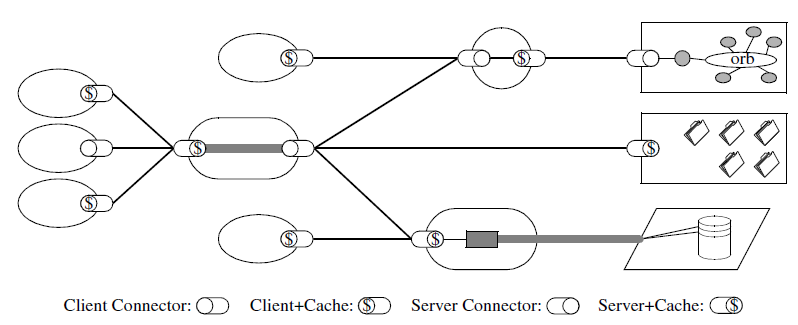
\includegraphics[width=\textwidth]{../images/background/Uniform-Layered-Client-Cache-Stateless-Server.png}
	\caption{Uniform-Layered-Client-Cache-Stateless-Server \cite{Fielding2000} }
	\label{fig:Uniform-Layered-Client-Cache-Stateless-Server}
 \end{figure}
\end{center}

\subsubsection{Summary}
Notion of independence was mentioned above in this section quite many times.
This is because REST itself is a high-level style that could be implemented
using any different technology and your favourite programming language. It was initially described in the context
of HTTP, but it is not limited to that protocol. 
You can use all your creativity in a system design and you are only limited with a small amount of abstract constraints. 
 RESTful applications maximize the use of the existing, well-defined interface
and other built-in capabilities provided by the chosen network protocol,
and minimize the addition of new application-specific features on top of
it\cite{rest_brief_intro}. Therefore RESTful Web services seamlessly integrate with the
Web and are straightforward and simple way of achieving a global network of
smart things.

